\begin{SingleSpace}
\chapter{Introduction}
\vspace{0.5cm}
\chapterprecishere{``Any finite number divided by infinity is as near to nothing as makes no odds, so the average population of all the planets in the Universe can be said to be zero. From this it follows that the population of the whole Universe is also zero, and that any people you may meet from time to time are merely the products of a deranged imagination.''\par\raggedleft--- \textup{Douglas Adams}, The Restaurant at the End of the Universe}
\end{SingleSpace}
\vspace{0.5cm}

Lava planets are rocky, very hot, and orbit so close to their host stars that they are expected to be tidally locked to them. This means that they always present the same side to the star, so have a permanent day-side and night-side. This thesis investigates the question of what these properties mean for the atmosphere of the planet, particularly its circulation and composition. Tidally locked planets are very common and observable. Lava planets are particularly observable, especially for rocky planets.

Why are tidally locked planets important? Their unusual situation could  make them seem like oddities, unrelated to the majority of planets. On the contrary, Figure \ref{fig:tide-locked-population} shows that a large fraction of known exoplanets are expected to be tidally locked. It shows the stellar masses and semi-major axes for all exoplanets listed on the NASA Exoplanet Archive at the time of writing, with all the planets below the line expected to be tidally locked \citep{pierrehumbert2018review}.

\clearpage
\begin{figure}
  \centering
    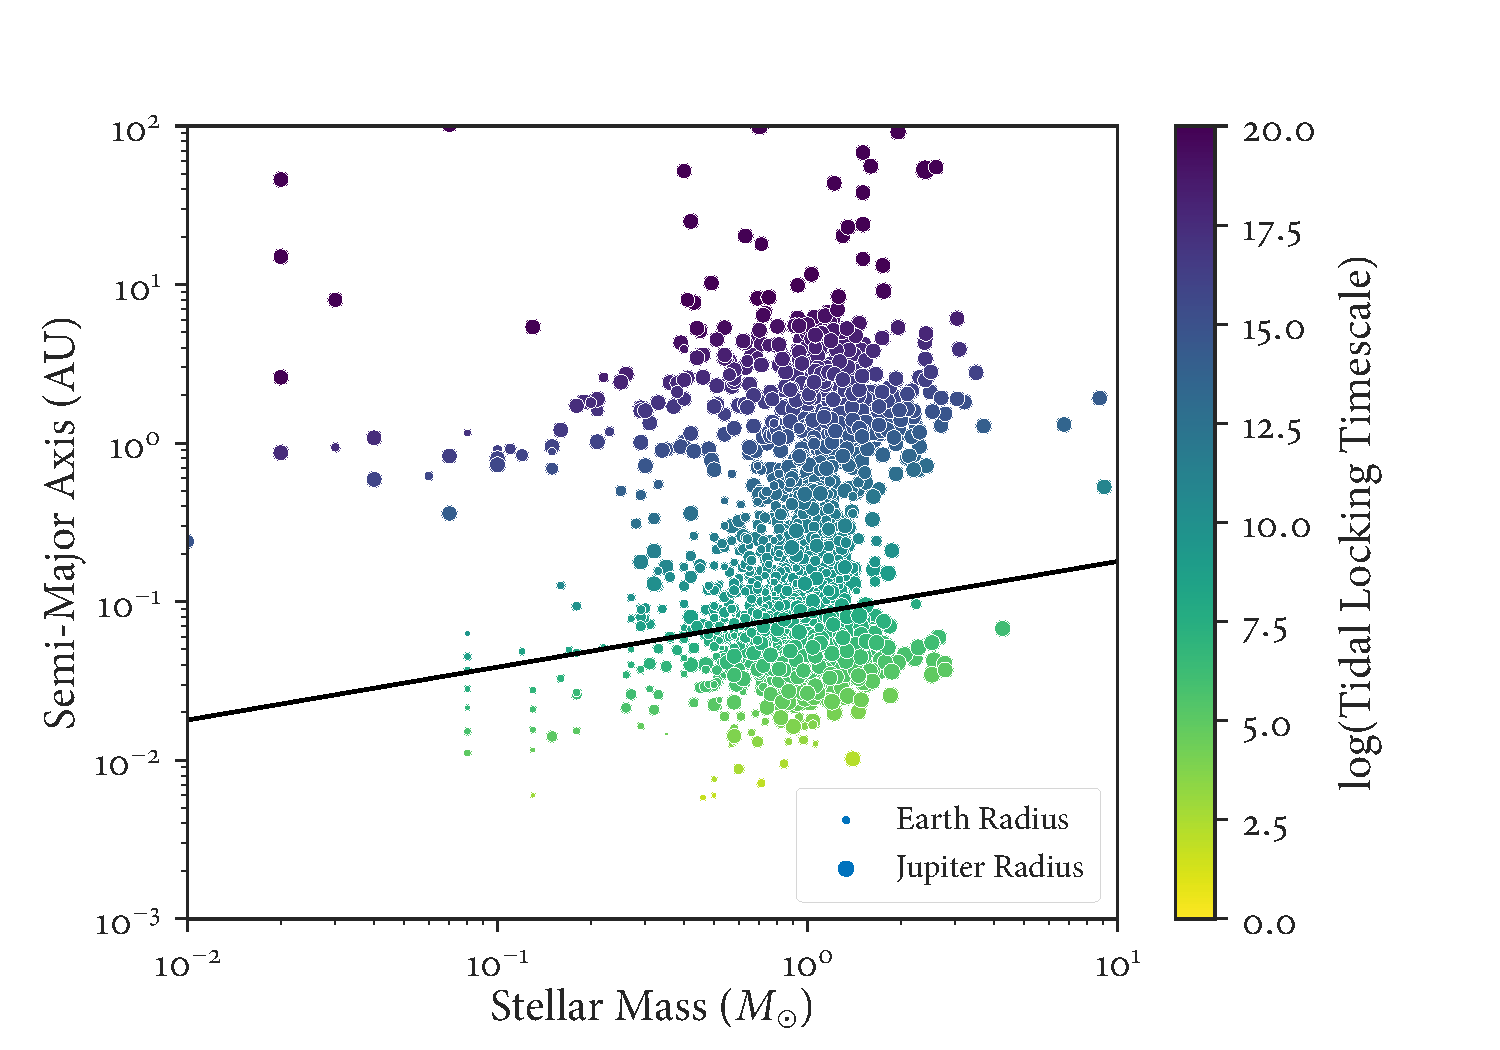
\includegraphics[width=1.0\textwidth]{figures/introduction/tide-locked-population.pdf}
    \caption{The population of known exoplanets plotted by semi-major axis and stellar mass. All the planets below the line have a timescale to reach a tidally locked state of less than 0.1 billion years, so are expected to be in this state.}
    \label{fig:tide-locked-population}
\end{figure}
\clearpage

 These planets are also generally more easily characterised than the others, giving larger signals for spectroscopy when they transit their stars. This tendency may have created a detection bias, where close-in exoplanets are more likely to be detected so it appears that a greater fraction are tidally locked than is actually the case. Even if this is true, it does not detract from the relevance of tidally locked planets -- we can only study planets we know about!

In Chapter 1, I discuss the concept of a ``lava planet'' and review the literature of discovery, characterisation, and modelling of such planets. I aim to introduce the scientific concepts and questions that I will address through the rest of the thesis.

In Chapter 2, I discuss the theoretical work I did to understand the global circulation of tidally locked planets in general. In the course of trying to understand simulations of tidally locked lava planets, we found that there was not a full understanding of key features of their circulation. I explain how I used a two-dimensional model to represent the atmosphere of a tidally locked planet, and demonstrated that the equatorial jet that forms affects the global circulation and temperature pattern. This was key to our work on lava planets, but was applicable to any tidally locked planet.

Chapter 3 follows Chapter 2

In Chapter 3, I introduce the model I used to simulate three-dimensional planetary atmospheres, the General Circulation Model (GCM) Exo-FMS. Developing this model formed a large part of the work of my DPhil. I discuss the structure I developed, and the physical processes represented within it. I focus on the particular challenges of simulating tidally locked lava planets, and defer many technical details to Appendix A.

In Chapter 4, I discuss my first project using the simulations discussed in Chapter 3, to interpret observations of a lava planet.

Chapter 5 follows Chapter 4, and shows how in collaboration with Graham Lee we simulated dynamic, radiatively active clouds on 55 Cancri e in order to answer the questions raised by Chapter 4 on the effect of clouds in its atmosphere.

In the Conclusion, I summarise my work on the global circulation of tidally locked planets, and its relevance for 55 Cancri e.



% \bibliographystyle{unsrtnat}
% \bibliography{../references.bib}
